The results presented in this analysis were obtained from a sample of minimum-bias and ultra-central lead-lead collisions at $\sqrt{s_{\text{NN}}}=5.02$ TeV recorded by ATLAS in 2015 (Run 2). The corresponding integrated luminosity are approximated $22-470 \mu b^{-1}$. The measurements were performed using the ATLAS inner detector and forward calorimeters. The inner detectors covers the complete azimuthal range and extends over the pseudorapidity region $|\eta|<2.5$. The inner detector silicon tracker, used in this analysis for track reconstruction, consists of layers of pixel and microstrip detectors (SCT) immersed in a 2 T axial magnetic field. An additional pixel layer, the "Insertable B Layyer" (IBL) installed between Run 1 and Run 2 (2013-2015), is used in the 5.02 TeV Pb+Pb measurements. The MBTS system detects charged particles over $2.1<|\eta|<3.9$ using two hodoscropes of counters positioned at $z=\pm 3.6$ m. The forward calorimeters (FCal) use liquid argon with copper tungsten absorbers to perform both the electromagnetic and hadronic energy measurements with copper-tungsten/liquid argon technology, and also provide complete coverage in azimuthal for $3.2<|\eta|<4.9$. The trigger system was used to select minimum-bias lead-lead collisions. It required a coincidence of signals recorded in both zero-degree calorimeters (ZDC), located symmetrically at $z=\pm 140$ m, and in the minimum-bias trigger scintillator (MBTS, only used in Run 1) counters at $z=\pm 3.6$ m.



\subsection{Triggers}
The minimum-bias triggers for 5.02 TeV Pb+Pb collisions are:
\begin{itemize}
\item \verb|HLT_mb_sptrk_ion_L1ZDC_A_C_VTE50|
\item \verb|HLT_noalg_mb_L1TE50|
\end{itemize}
where the major difference is Level-1 total energy $\verb|TE|$: $\verb|VTE50|$ requires total energy less than 50 GeV while $\verb|TE50|$ larger than 50 GeV; $\verb|sptrk|$ requires at least 1 reconstructed track at the HLT level, and $\verb|L1ZDC_A_C|$ requires one hit in both sides of ZDC. These two requirements will clean up most diffractive events. In any case, this measurement stops at $80\%$ centrality, which means the contributions from diffractive events are minimal.

To enhance the statistics in ultra-central events, ultra-central collision (UCC) triggers are used:
\begin{itemize}
\item \verb|HLT_hi_th1_ucc_L1TE10000|
\item \verb|HLT_hi_th2_ucc_L1TE10000|
\item \verb|HLT_hi_th3_ucc_L1TE10000|
\item \verb|HLT_hi_th1_ucc_L1TE12000|
\item \verb|HLT_hi_th2_ucc_L1TE12000|
\item \verb|HLT_hi_th3_ucc_L1TE12000|
\item \verb|HLT_hi_th1_ucc_L1TE14000|
\item \verb|HLT_hi_th2_ucc_L1TE14000|
\item \verb|HLT_hi_th3_ucc_L1TE14000|
\end{itemize}
where $\verb|L1TEX|$ denotes the minimum L1 total energy cut and $thX$ corresponds to the various minimum FCal Calorimeter $E_{\text{T}}$ cut at the HLT level:
\begin{itemize}
\item \verb|th1|: online FCal $E_{\text{T}}>4.172$ TeV;
\item \verb|th2|: online FCal $E_{\text{T}}>4.326$ TeV;
\item \verb|th3|: online FCal $E_{\text{T}}>4.500$ TeV;
\end{itemize}

Fig.~\ref{fig:evtSel_UCC_sts} shows the FCal $E_{T}$ distributions seeded by two major UCC triggers, compared with those seeded by MinBias triggers. UCC triggers collected more than 20 times statistics compared with MinBias triggers in the ultra-central collisions. Meanwhile, as seen in these plots, the turn-on curves of UCC trigger efficiency are very sharp, which means small selection bias. The impact from trigger efficiency will be discussed in details in Sec.~\ref{sec:sys}.
\begin{figure}[H]
\centering
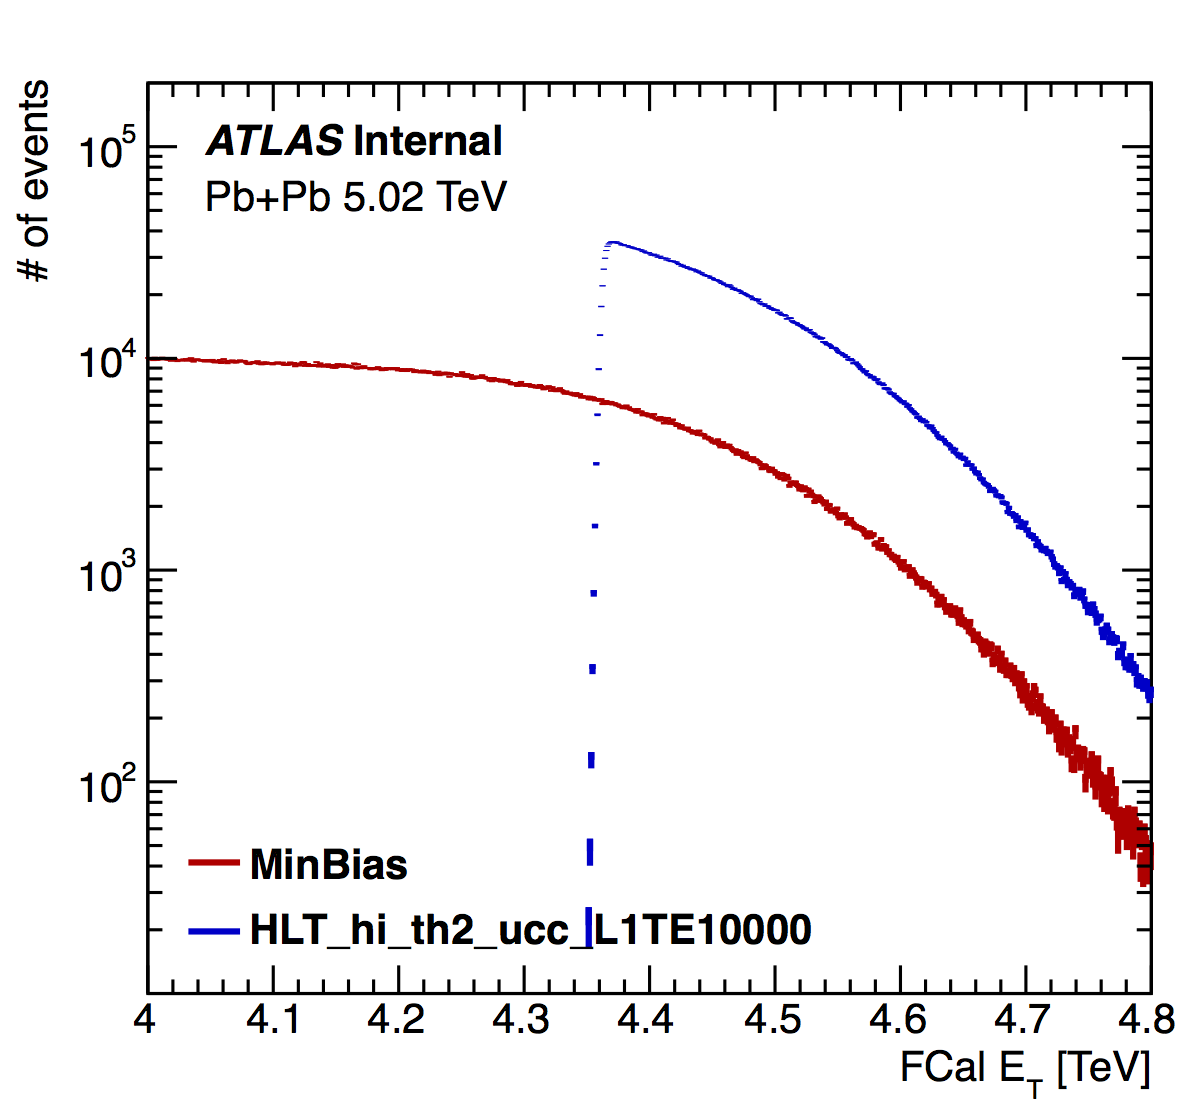
\includegraphics[width=.45\linewidth]{figs/sec_evtSel/PbPb502/UCC_trigSts_3.png}
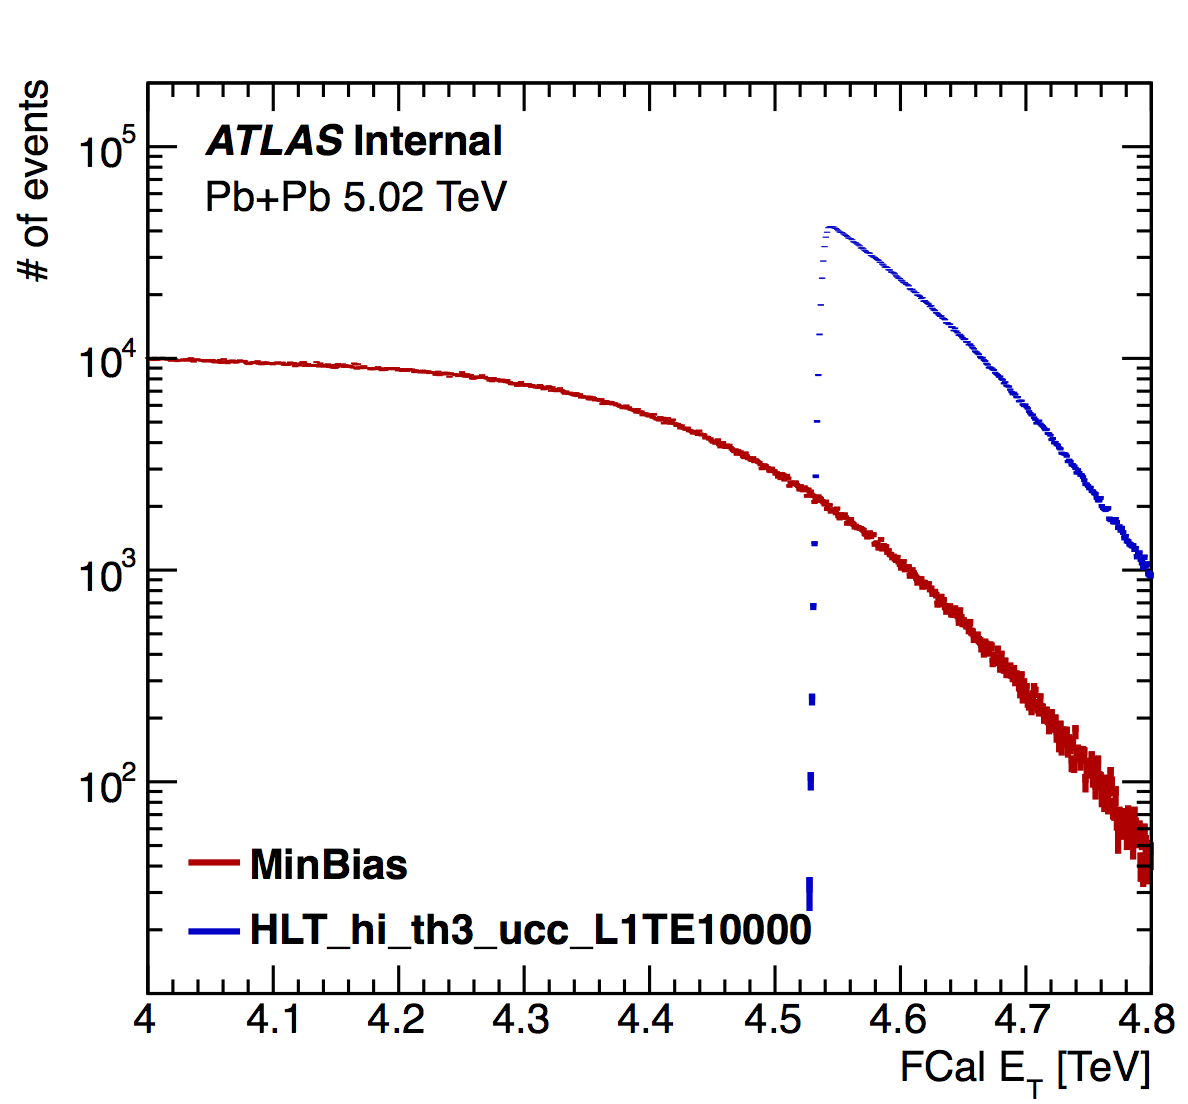
\includegraphics[width=.45\linewidth]{figs/sec_evtSel/PbPb502/UCC_trigSts_4.png}
\caption{FCal $E_{T}$ distribution for two major UCC triggers (red points), compared with MinBias trigger (blue points).}
\label{fig:evtSel_UCC_sts}
\end{figure}



\subsection{Event selection}
The reconstruction version of the data set is $\verb|data15_hi.XXX.physics.MinBias.recon.AOD.r7874|$. The event selections for 5.02 TeV Pb+Pb events are:
\begin{itemize}
\item Pass good run list (GRL): \url{https://twiki.cern.ch/twiki/bin/viewauth/Atlas/HeavyIonRunList};
\item Have a primary reconstructed vertex;
\item Events with detector error tags removed:
\begin{itemize}
\item LAr error;
\item Tile error;
\item SCT error;
\item Incomplete events;
\end{itemize}
\item Vertex position cut: $|z_{vtx}|<100$ mm;
\item $0\%\leq\text{centrality}<80\%$;
\item Pileup rejection: \url{https://twiki.cern.ch/twiki/bin/view/Main/HIAnalysisTools#HI\_Pileup\_Tool\_Working};
\end{itemize}
where the definition of centrality will be discussed shortly. In this analysis we are cutting the vertex position at $100$ mm instead of $150$ mm (in previous Pb+Pb analysis). This is because multiplicity distribution along $\eta$ changes with the $z_{vtx}$ position, and in previous measurements it is not an issue since all the particles in $|\eta|<2.5$ are used to calculate the cumulant. However, with the 3-subevent cumulant method, two subevents are defined with the range $2.5/3<|eta|<2.5$, which is closer to the edges of the Inner Detector. In order to avoid introducing large multiplicity fluctuations in these two subevents, we further constrain the vertex position to $100$ mm, and we will not loose much statistics with this tighter cut.

In the 2015 Pb+Pb run, the luminosity conditions provided by the LHC result in an average probability of $0.1\%$ that an event contains two or more Pb+Pb collisions (pileup). The pileup events are suppressed by only using the tracks from primary vertex (in fact, in Pb+Pb, only one primary vertex is reconstructed). The remaining pileup events are further suppressed based on the correlation between the ZDC and FCal. This signal in the ZDC is calibrated to the number of detected neutrons $N_n$ based on the location of the peak corresponding to a single neutron.

Fig.~\ref{fig:evtSel_pu} shows the procedure of pileup rejection and its performance. The left plot shows the correlation between number of neutrons in the ZDC and total transverse energy $E_T$ in the FCal. The "banana"-shaped main band (green) mainly contains events with a single vertex. While in a pileup event, both the number of neutrons and FCal $\sum E_T$ are larger than a single event, and this is indicated by the events in the "grass" (purple) region above the main band. To clean up the pileup, one way is by applying a linear cut on the correlation map, indicated by the black straight line, and another way is cutting off $0.1\%$ of the events in the tails of $N_\text{neutrons}$ distribution in each FCal $E_{T}$ slice, indicated by the red curve. In this analysis, we will use the red curve as the default cut. The right plot shows the performance of the two pileup rejection methods just mentioned. The Y-axis shows the fraction of rejected pileup events out of all the pileup events. The rejection rate is low at low FCal $E_{T}$, this is because the band for pileup events most overlaps with the main band for single events. However, since the fraction of pileup events is very low in peripheral collisions, the low rejection rate has no impact on the results. On the other hand, the rejection rate reaches $100\%$ in ultra-central collision, where the fraction of pileup event is high, meaning that almost all the pileup events are rejected using the HI pileup rejection tool.
\begin{figure}[H]
\centering
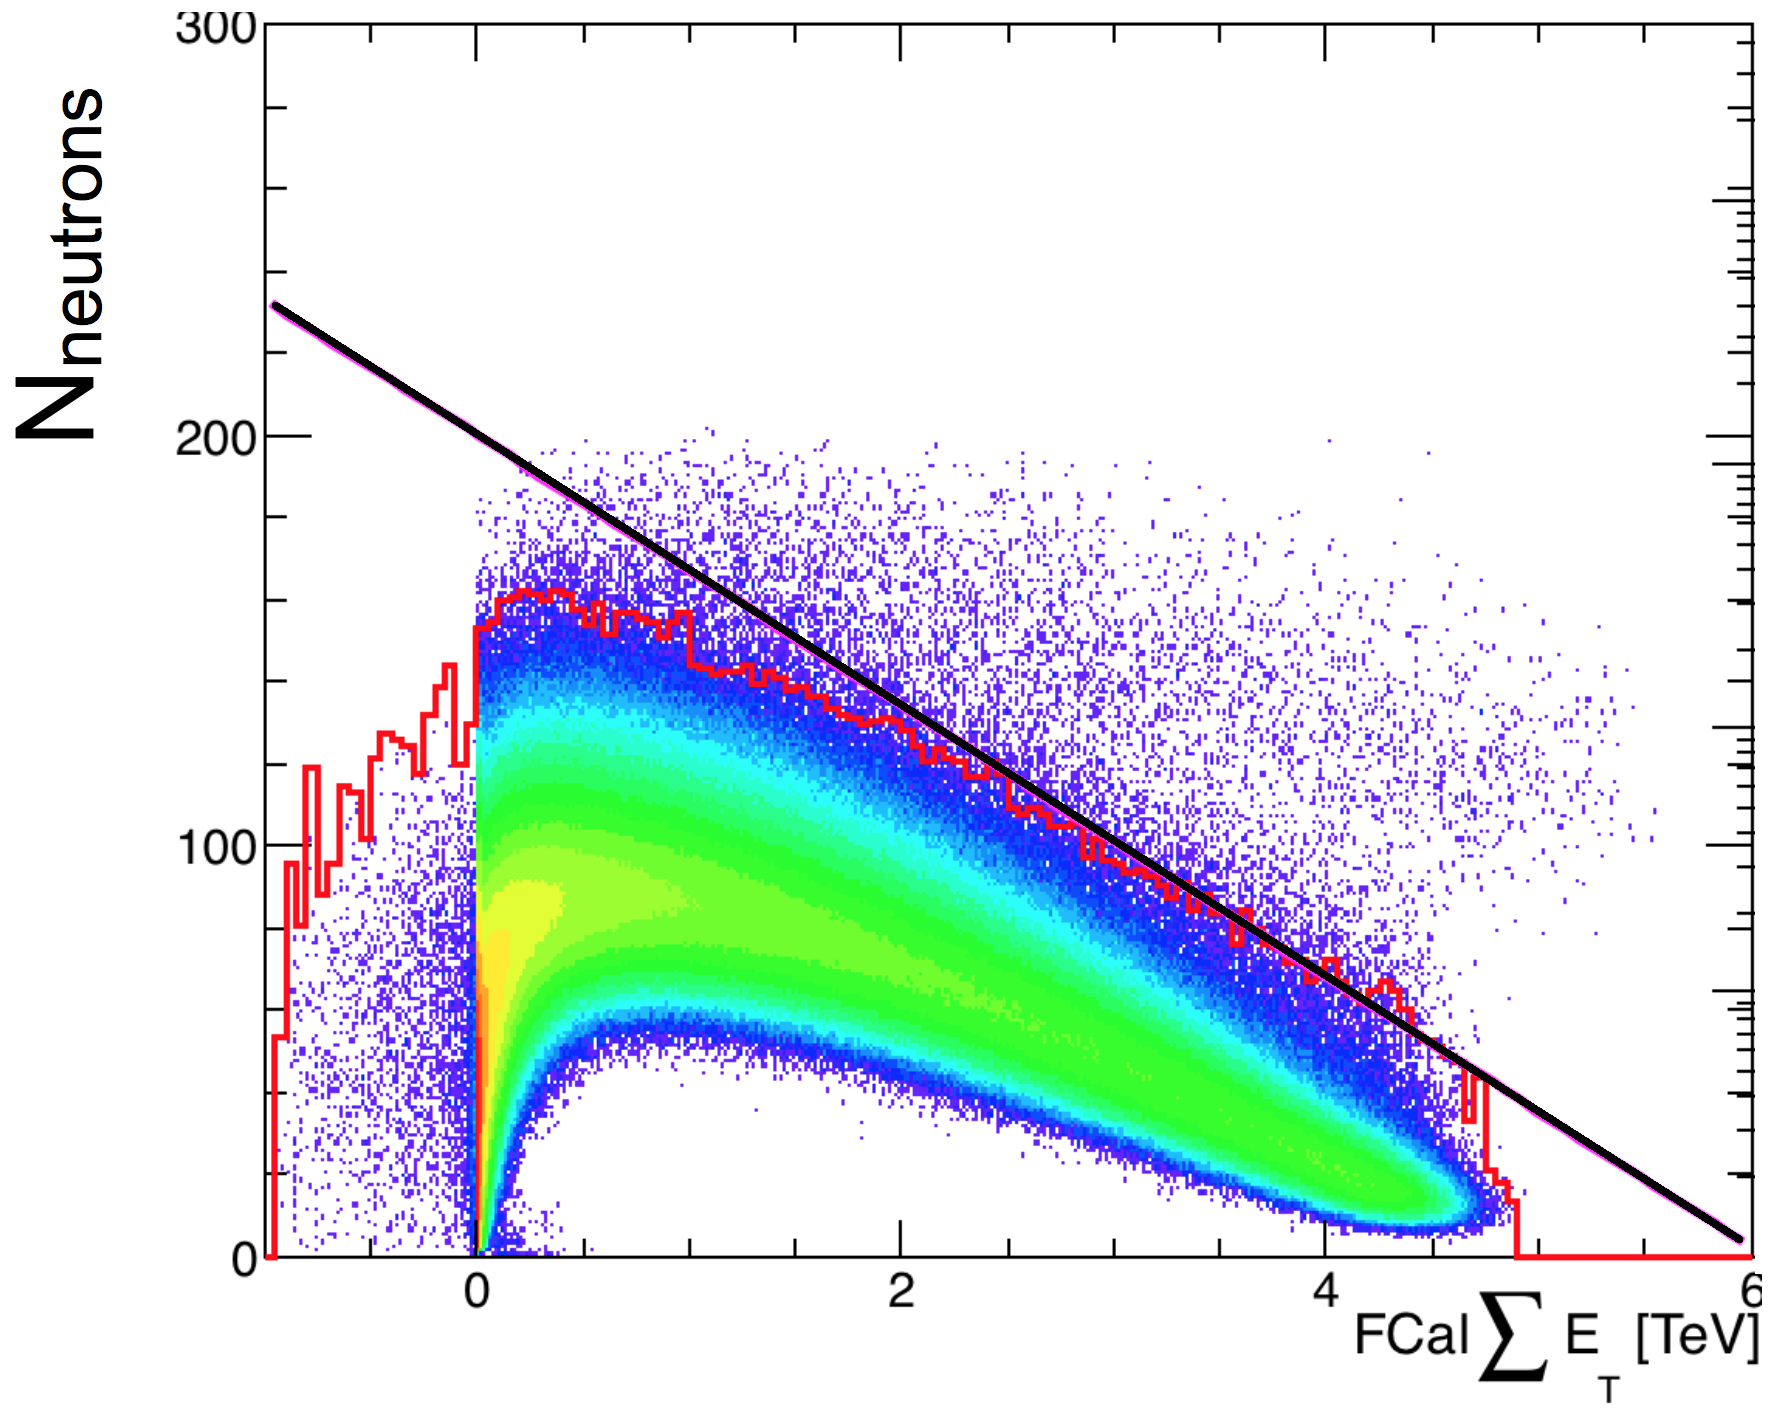
\includegraphics[width=.45\linewidth]{figs/sec_evtSel/PbPb502/pu_corr.png}
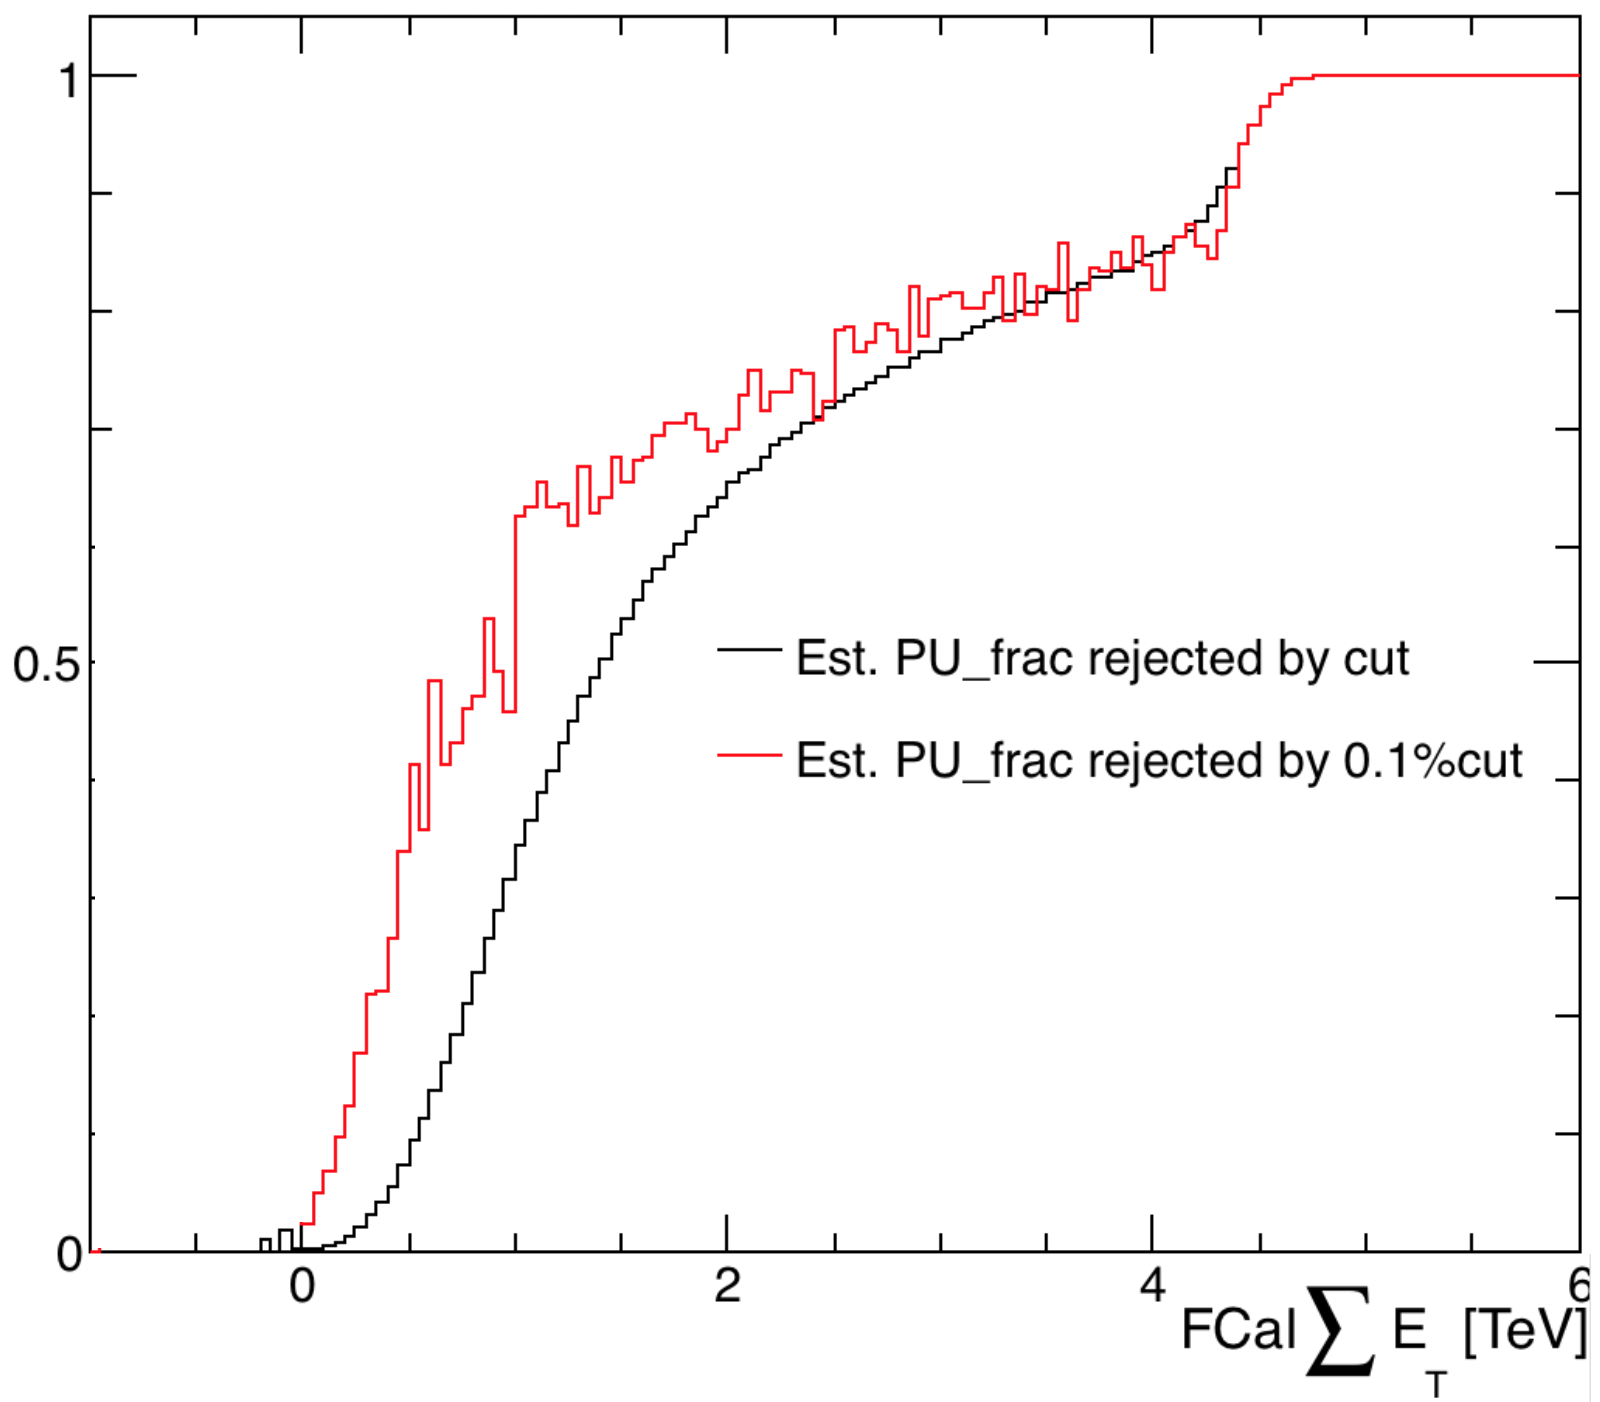
\includegraphics[width=.45\linewidth]{figs/sec_evtSel/PbPb502/pu_perf.png}
\caption{Left plot shows the correlation between calibrated number of neutrons in the ZDC and FCal $\sum E_T$. Right plot shows the fraction of rejected pileup events in all pileup events. Two rejection criteria are shown: a linear cut and $0.1\%$ cut.}
\label{fig:evtSel_pu}
\end{figure}

Fig.~\ref{fig:evtSel_pu_rate} illustrates the FCal sum $E_T$ distribution before and after this pileup cut, as well as the fraction of events that are rejected as a function of FCal sum $E_T$. As expected, the rejection rate is $<0.2\%$ for FCal $E_T<4.5$ TeV, and increases toward 1 quickly as FCal $E_T$ increases.
\begin{figure}[H]
\centering
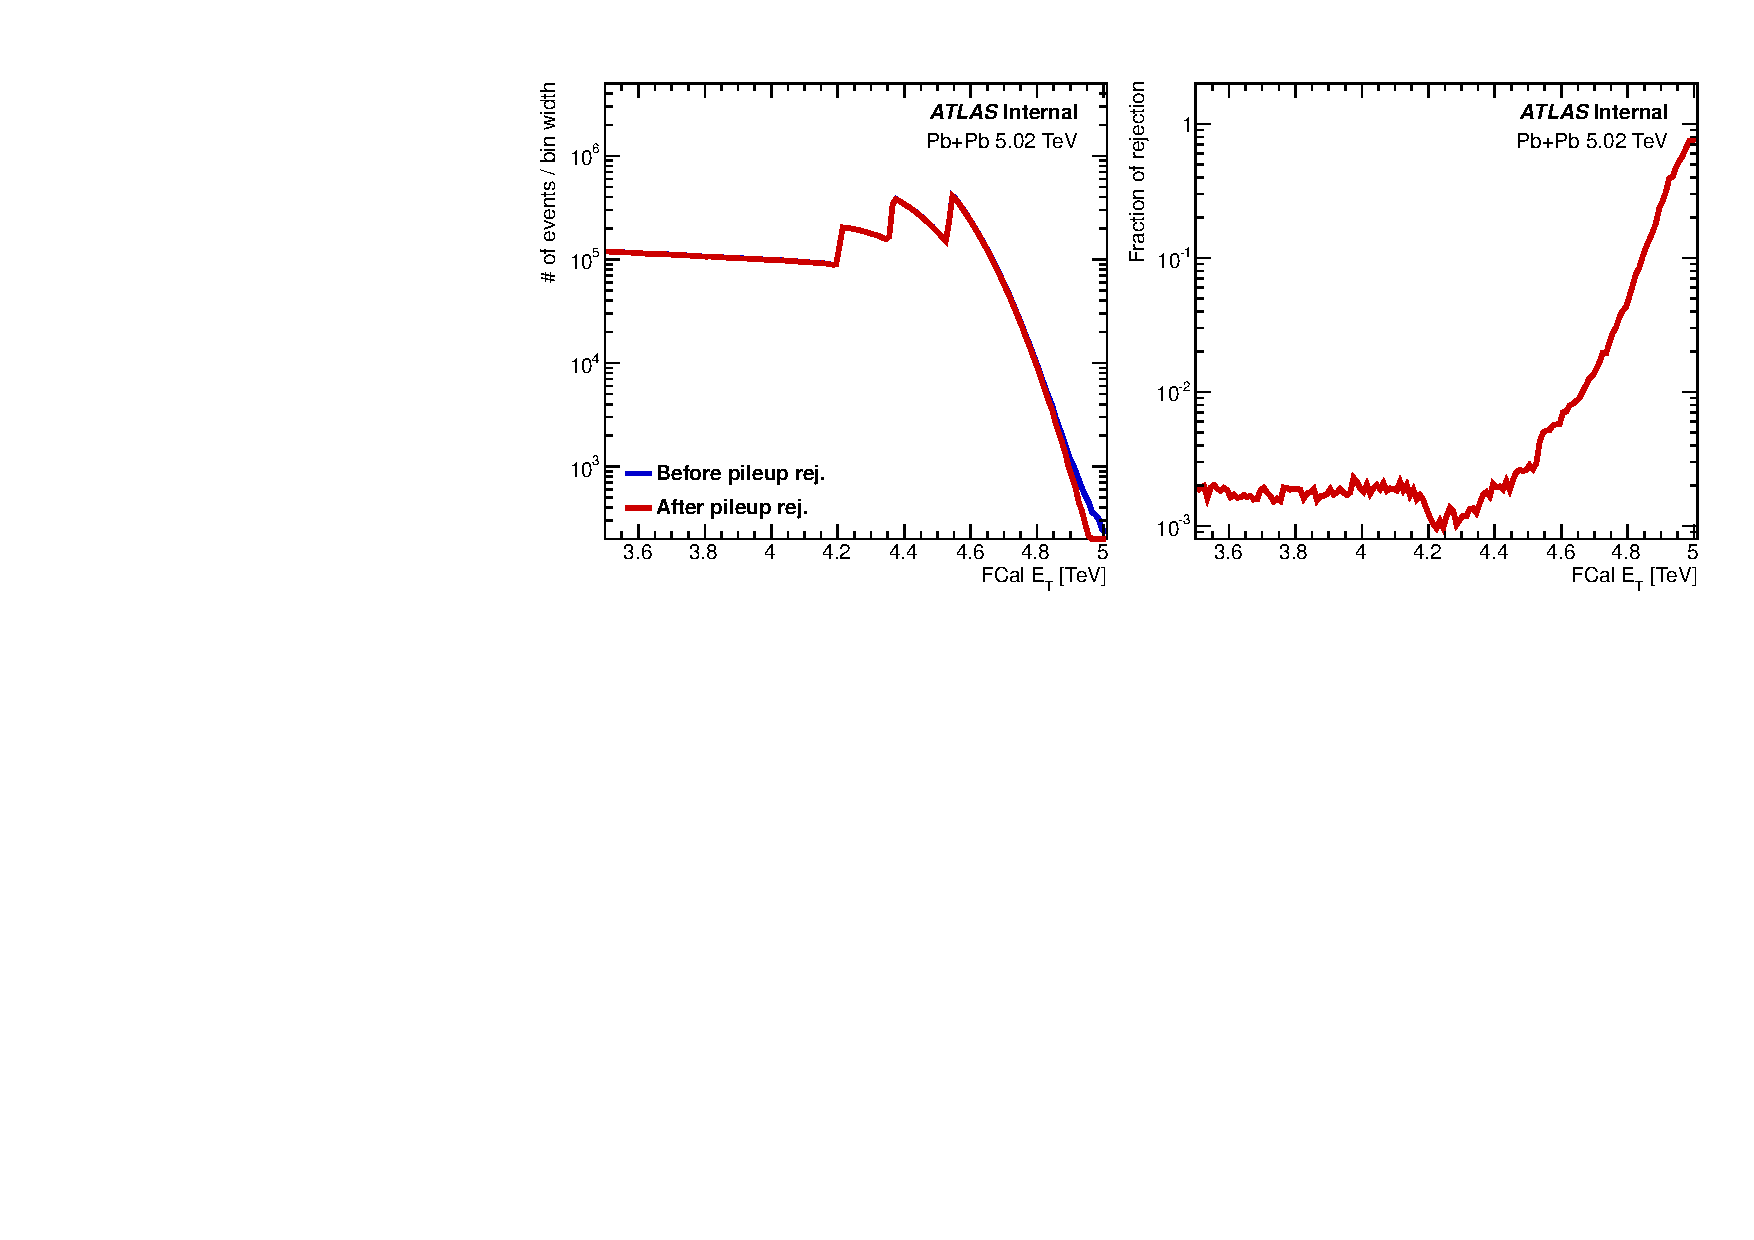
\includegraphics[width=.9\linewidth]{figs/sec_evtSel/PbPb502/puCut.pdf}
\caption{Left plot shows the FCal sum $E_T$ distribution before and after applying the HI pileup tool. Right plot shows the fraction of events that are rejected by this tool, as a function of FCal sum $E_T$.}
\label{fig:evtSel_pu_rate}
\end{figure}

Furthermore, in order to further suppress the residual pileup events, an additional cut has been applied on the correlation map between FCal $E_{T}$ and efficiency corrected reconstructed number of tracks $N_{ch}$. Fig.~\ref{fig:evtSel_addPuCut} shows the correlation froms MinBias events (left), and UCC events collected with one of the UCC triggers (right) as a demonstration. Since pileup events have relatively larger FCal $E_{T}$ than normal events, the pileup events should fall under the main correlation band. From the correlation map, some "grass" is indeed observed. To determine the cut, a Gaussian fitting is applied to the $N_{ch}$ distribution for each FCal $E_{T}$ slice, and the events beyond $5 \sigma$ are rejected (indicated by the red dots). To reach the high FCal $E_{T}$ region, where the performance of Gaussian fit is poor (because of the additional structure from pileup events), a linear cut is determined by fitting the red dots in the region FCal $E_\text{T}<4,7$ TeV. Events below this linear cut are rejected.
\begin{figure}[H]
\centering
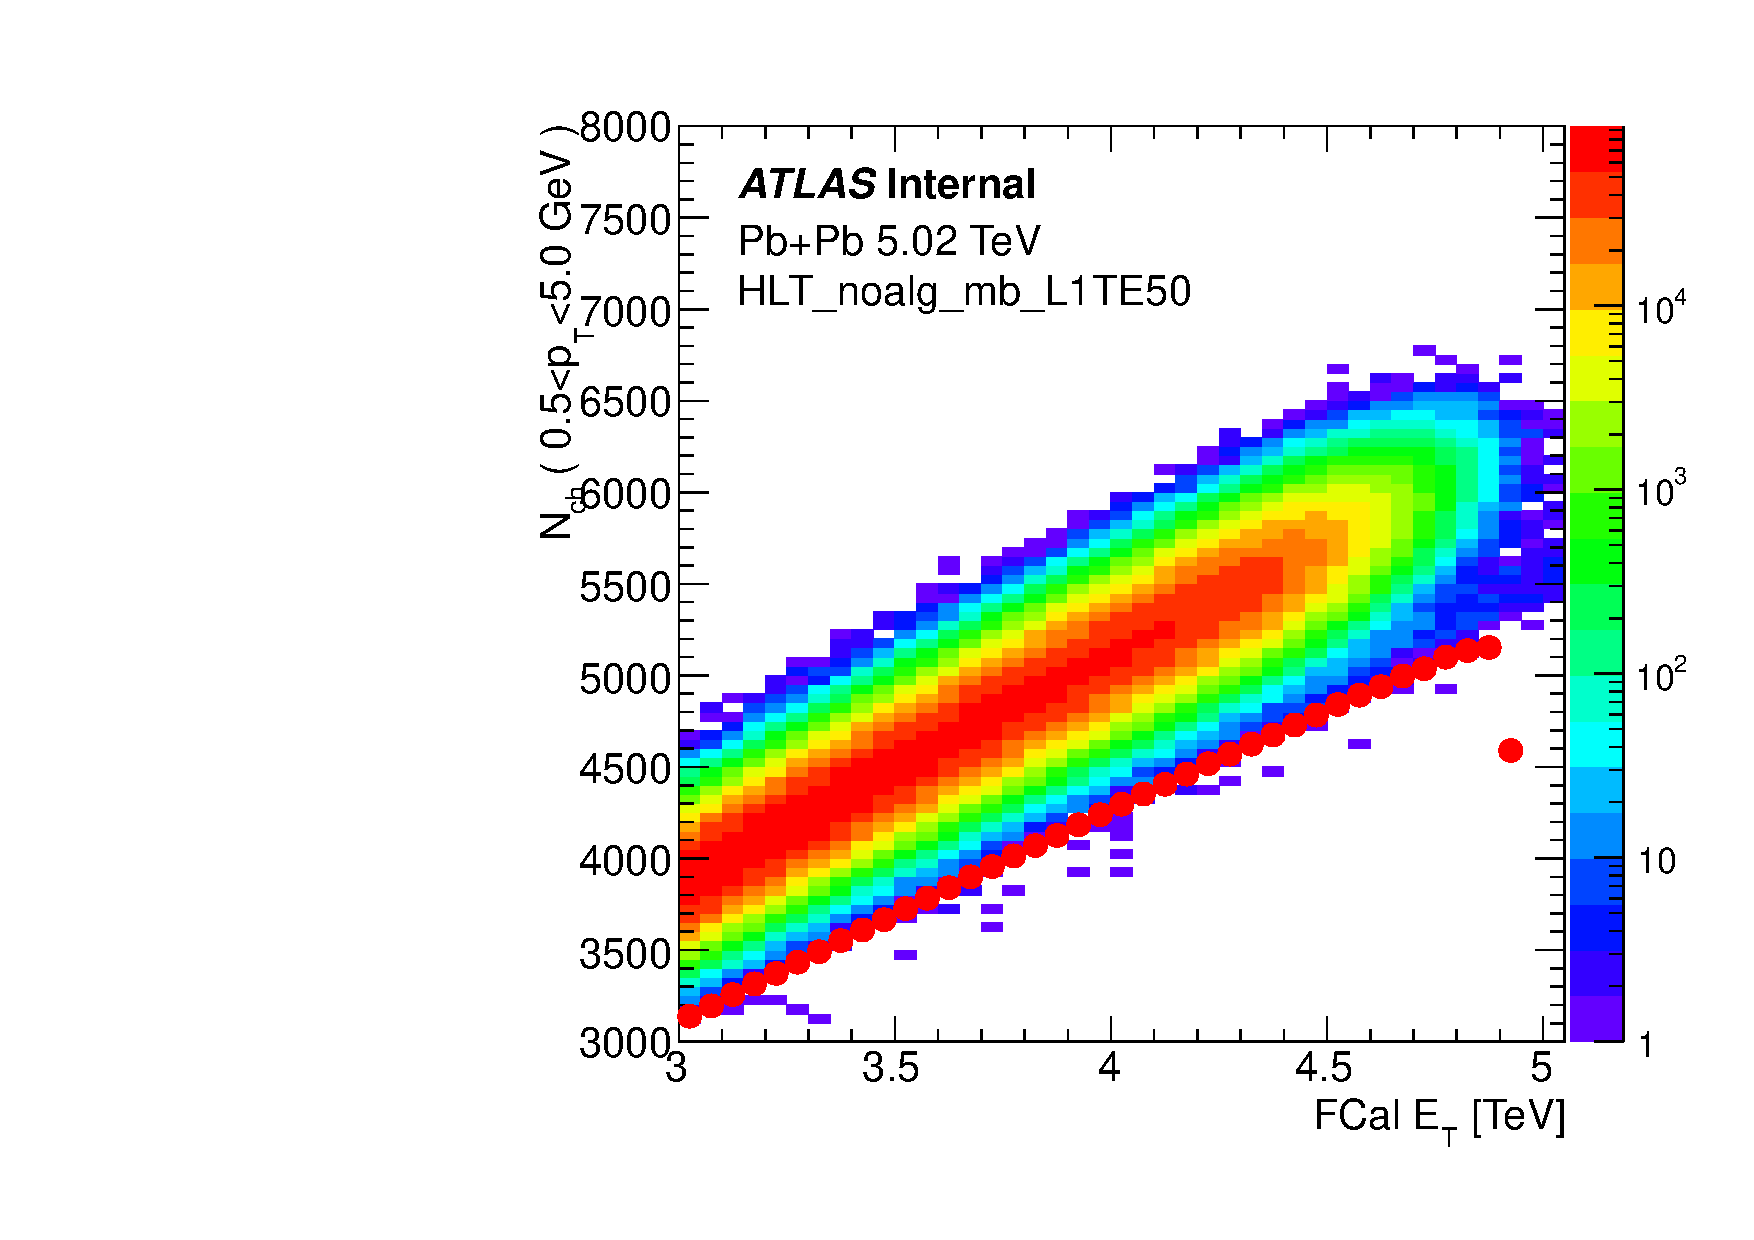
\includegraphics[width=.45\linewidth]{figs/sec_evtSel/PbPb502/puCut_1.pdf}
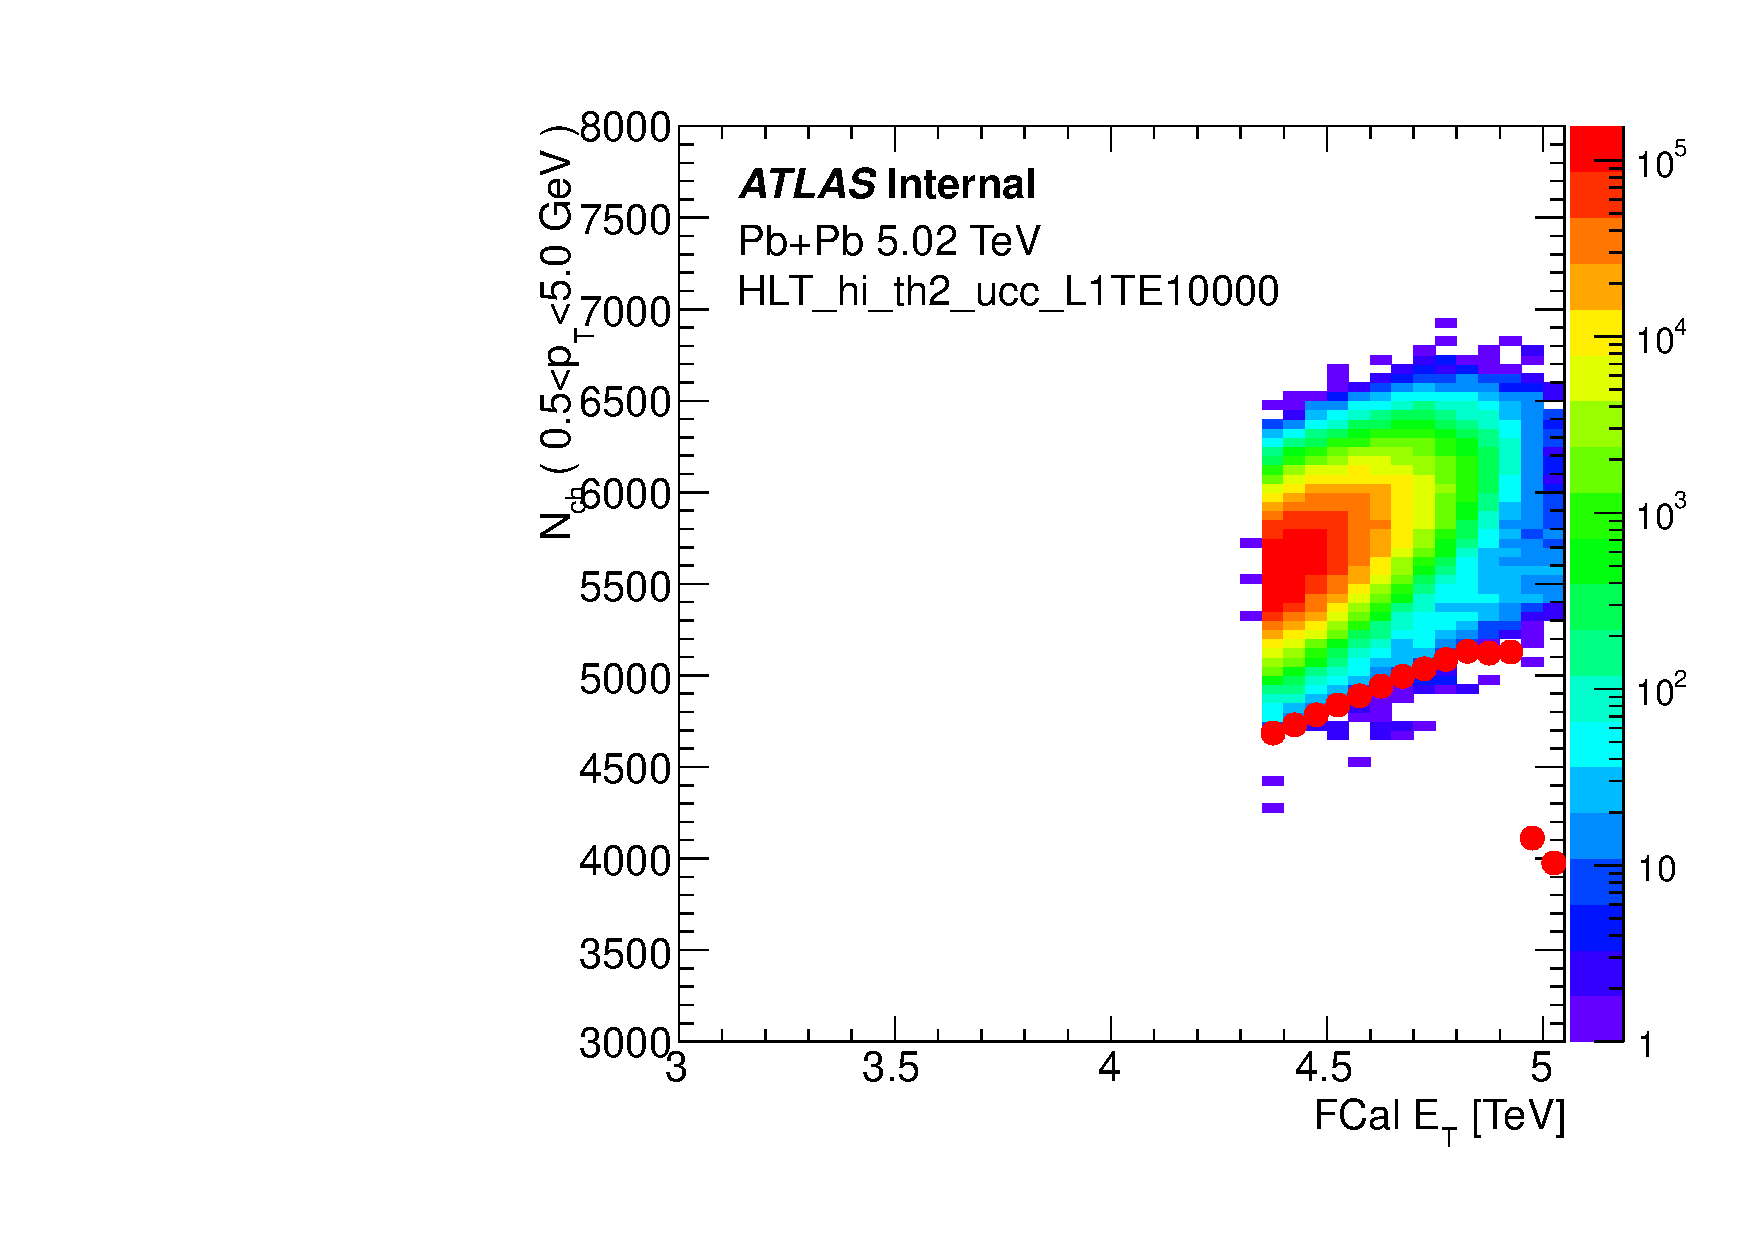
\includegraphics[width=.45\linewidth]{figs/sec_evtSel/PbPb502/puCut_3.pdf}
\caption{Correlation between FCal $E_{T}$ and $N_{ch}$ in the ultra-central collisions. The red dots indicate the $5 \sigma$ position of the Gaussian fit in each $N_{ch}$ slice at fixed FCal $E_{T}$. The actual cut is a linear fit of the red points in order to reach the largest FCal $\sum E_T$ region.}
\label{fig:evtSel_addPuCut}
\end{figure}



\subsection{Centrality}
The details of centrality cuts are documented here: \url{https://twiki.cern.ch/twiki/bin/view/AtlasProtected/HeavyIonAnalysis2015#NEW\_Centrality\_Recommendations\_f}. The Pb+Pb event centrality is characterized using the total transverse energy ($\sum E_T$) deposited in the FCal detector at the electromagnetic energy scale. An analysis of this distribution after all triggers and event selections gives an estimation of the fraction of the sampled non-Coulomb inelastic cross-section to be $85\%\pm1\%$. This estimate is obtained from a shape analysis of the measured FCal $\sum E_T$ distributions compared with a convolution of proton-proton data with a Monte Carlo Glauber calculation. The FCal $\sum E_T$ distribution is then divided into a set of $1\%$ percentile bins, together with a bin defined for the $0.1\%$ most central events. The uncertainty associated with the centrality definition is evaluated by varying the effect of trigger and event selection inefficiencies as well as background rejection requirements in the most peripheral FCal $\sum E_T$ interval.

The centrality interval and corresponding number of participants $N_{\text{part}}$ estimated from Glauber model are listed in Table.~\ref{table:centrality_run2}
\begin{table}[ht]
\begin{tabular}{c c c c c c c c c}
\hline\hline
Centrality        &  0-5\% & 5-10\% & 10-15\% & 15-20\% & 20-25\% & 25-30\% & 30-35\% & 35-40\% \\
$N_{\text{part}}$ &  384.5 & 333.1  & 285.2   & 242.9   & 205.6   & 172.8   & 144.1   & 118.8   \\
Centrality        &40-45\% & 45-50\%& 50-55\% & 55-60\% & 60-65\% & 65-70\%  & 70-75\%& 75-80\% \\ 
$N_{\text{part}}$ &96.6    & 77.4    & 60.9    & 47.0    & 35.2    & 25.8     & 18.3   & 12.5 \\
\hline
\end{tabular}
\centering
\caption{Centrality intervals and corresponding number of participants $N_{\text{part}}$ estimated from Glauber model in Run 2.}
\label{table:centrality_run2}
\end{table}

